\chapter{Обзор аналогов}\label{ch:0}

На сегодняшний день мне известны лишь два случая обслуживающих манипуляторов. Первый в заведении \textit{Cafe X}, расположившемся в Сан-Франциско(см. рис. \ref{fig:1_0}).
\begin{figure}[h!]
	\centering
	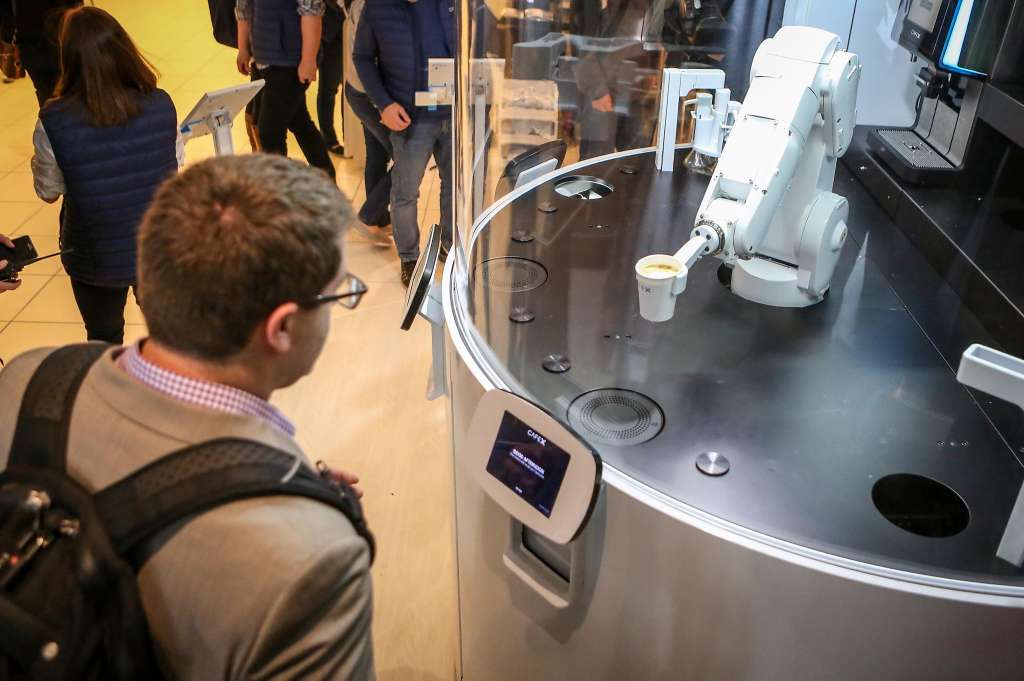
\includegraphics[scale=0.35]{intro/cafe_x}
	\caption{Манипулятор, обслуживающий Cafe X}
	\label{fig:1_0}
\end{figure}

Второй робот находится в Токио в кафе под названием \textit{Henna}.
\begin{figure}[h!]
	\centering
	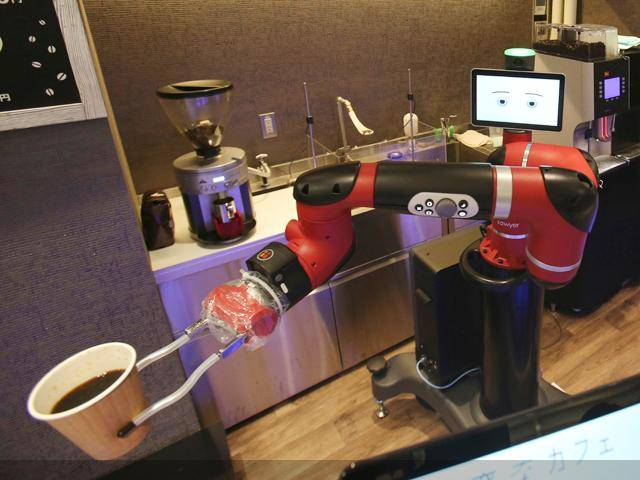
\includegraphics[scale=0.35]{intro/henna_cafe}
	\caption{Манипулятор, обслуживающий Henna Cafe}
	\label{fig:1_1}
\end{figure}

Как бы то ни было, но оба эти робота выполняют роль баристы. На самом деле их экономическое преимущество по сравнению с обычными торговыми автоматами неочевидно, в представленных примерах, манипуляторы выполняют, скорее, роль аттракциона, нежели действительно способствуют автоматизации рутинных процессов.

Если бы была возможность встраивать роботизированную систему, способную не только наливать кофе, но и формировать заказы из различных блюд, а также способную выполнять работу продавцов значительно быстрее, это могло бы сэкономить бизнесу серьезные суммы денег на содержании штата, при этом увеличив пропускную способность заведений.